\documentclass[12pt]{article}
\usepackage{times}
\usepackage{amsmath}
\usepackage{amsfonts}
\usepackage{graphicx}
\usepackage[usenames, dvipsnames]{color}
\usepackage{multirow}
\usepackage{multibib}
\usepackage{tabularx, booktabs}
\usepackage{longtable}
\usepackage{caption}
\usepackage{colortbl}
\usepackage{siunitx}
\usepackage{url}
\usepackage{hyperref}

\usepackage[top=1in, bottom=1in, left=1in, right=1in]{geometry}

\definecolor{darkgreen}{RGB}{0, 125, 0}
\definecolor{orange}{RGB}{255, 125, 125}
\definecolor{darkgray}{RGB}{64, 64, 64}
\newcolumntype{S}{>{\hsize=.3\hsize}X}

\topmargin 0.0cm
\oddsidemargin 0.2cm
\textwidth 16cm
\textheight 21cm
\footskip 1.0cm

\newenvironment{sciabstract}{%
\begin{quote} \bf}
{\end{quote}}

\title{Title}
\date{}

\author
{
Chen Fu$^{1}$\\
Others$^{2}$
\\
\\
\normalsize{$^{1}$Org1.}
\\
\normalsize{$^{2}$Org2.}
}

\begin{document}
\maketitle

\begin{abstract}
  Abstract gose here.
\end{abstract}


\section{Help}

% \subsection{Table}
\begin{table}
	\begin{tabularx}{\textwidth}{XXXX}
		\toprule
		table & a & b \\
		\midrule
    $\alpha$ & 1 & 2 \\
    $\beta$  & 2 & 3 \\
    $\gamma$ & 3 & 4 \\
		\bottomrule
	\end{tabularx}
	\caption
	{
		\label{tab:example}
    table's label
	}
\end{table}

\subsection{Formula}

\begin{align}
	a_t & = \arg\max\limits_{a}\left(Q(s,a)+u(s,a)\right)\\
	Q(s,a) & =\frac{\bar{L}}{L(s,a)/N(s,a)} \\
	u(s,a) & = C_pP(s,a)\frac{\sqrt{\sum_bN(s,b)}}{1+N(s,a)}
\label{eqn:select}
\end{align}

% \subsection{Figure}
\begin{figure}
\centering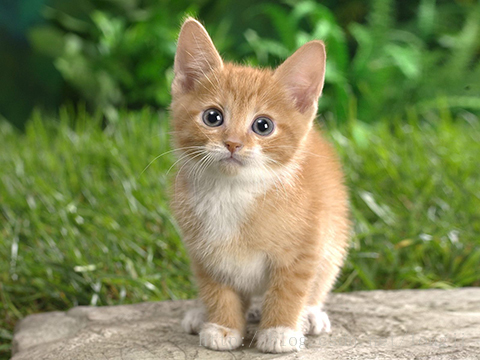
\includegraphics[height=0.36\textheight]{images/cat.jpeg}
\caption{
\label{fig:cat}
cute cat
}
\end{figure}

\subsection{Cite}
\begin{itemize}
\item \emph{References}: \cite{silver2017mastering}
\item \emph{Formula}: \ref{eqn:select}
\item \emph{Table}: \ref{tab:example}
\item \emph{Figure}: \ref{fig:cat}
\end{itemize}

\begin{enumerate}
\item \emph{Selection}: ...
\item \emph{Expansion}: ...
\item \emph{Simulation}: ...
\item \emph{Backpropagation}: ...
\end{enumerate}

\subsection*{No no. section}


\bibliographystyle{plain}
\bibliography{main}

\end{document}
